\problemname{Familiesammenkomst}
\begin{figure}[h!]
  \centering
  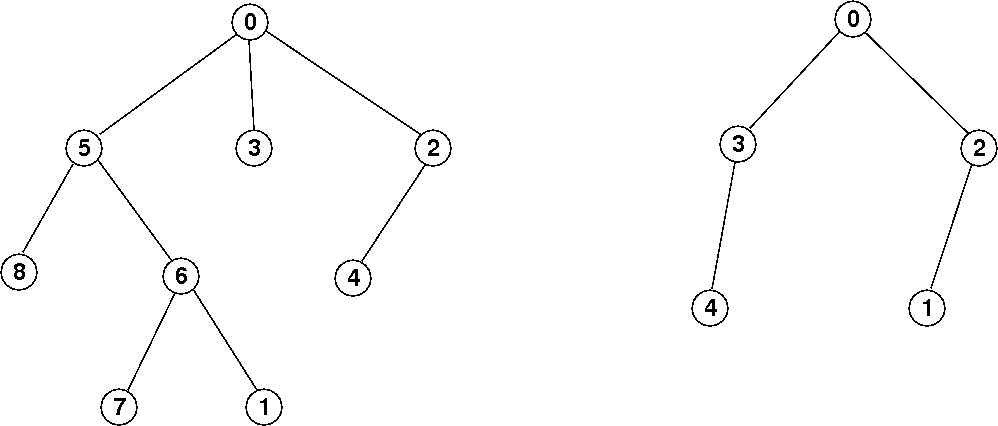
\includegraphics[width=16cm]{slakttraffen.png}
  \caption{Slægtstræerne for de to kørselseksempler.}
\end{figure}

Det er igen blevet tid til familiesammenkomst for Ida-Ottilia Isaksons efterkommere.
For enkelthedens skyld har man oprettet et slægtstræ og nummereret alle efterkommere fra $1$ til $N$; Ida-Ottilia selv har fået nummer~$0$.
Blandt de $M$ personer ved dit bord er der opstået en diskussion om, hvem der er den nærmeste slægtning, som er ane til alle ved bordet.
Skriv et program som beregner dette.

Programmet skal indlæse antallet af efterkommere, $N$, og derefter nummeret på hver persons forælder, hvilket naturligvis altid er mellem $0$ og $N$.
Derefter skal programmet indlæse antallet $M$ af personer ved bordet ($2 \le M \le N$) og nummeret på hver af dem.
Programmet skal så svare med nummeret på den person som er den nærmeste fælles ane, dvs.\ den nærmeste slægtning opad i træet som er forgænger til alle ved bordet.
Læg mærke til, at denne person ikke nødvendigvis selv sidder ved bordet.

\section*{Indlæsning}
På første linje i indlæsningen står tallene $N$ og $M$ ($2 \le M \le N \le 20$).
På anden linje står $N$ tal som beskriver hver persons forælder (alle mellem $0$ og $N$).
På tredje linje står $M$ tal som beskriver personerne ved bordet (alle mellem $1$ og $N$, uden dubletter).

\section*{Udskrift}
Programmet skal skrive et enkelt tal: nummeret på nærmeste fælles ane til personerne ved bordet.
